\documentclass[xcolor=dvipsnames]{beamer}
\usepackage[utf8]{inputenc}
\usepackage[IL2]{fontenc}
\usepackage[czech]{babel}
\usepackage{float}
\usepackage{listings}
\usepackage{amssymb}
\usepackage{amsmath}
\usepackage{mathtools}
\usepackage{url}
\usepackage{graphicx}
\usepackage{subfigure}
%\useoutertheme[subsection=false]{smoothbars}
\usetheme{Madrid}
\usecolortheme[named=OliveGreen]{structure}
%\usecolortheme[named=OliveGreen]{structure} 
%\usetheme[height=7mm]{Rochester} 
%\setbeamertemplate{items}[ball] 
%\setbeamertemplate{blocks}[rounded][shadow=true] 
%\useoutertheme{umbcfootline}
\beamertemplatenavigationsymbolsempty 
\title{Kolektivní investování}
\author{Marek Bryša, Jan Kovář}
\institute
{
Masarykova Univerzita\\
Přírodovědecká fakulta
}
\date{\today}

\begin{document}
  \frame{\titlepage}
  \section{Teoretická část}

	\section{Vybrané fondy v České republice}
		\begin{frame}{AXA investiční společnost, a.s.}
			\begin{center}
				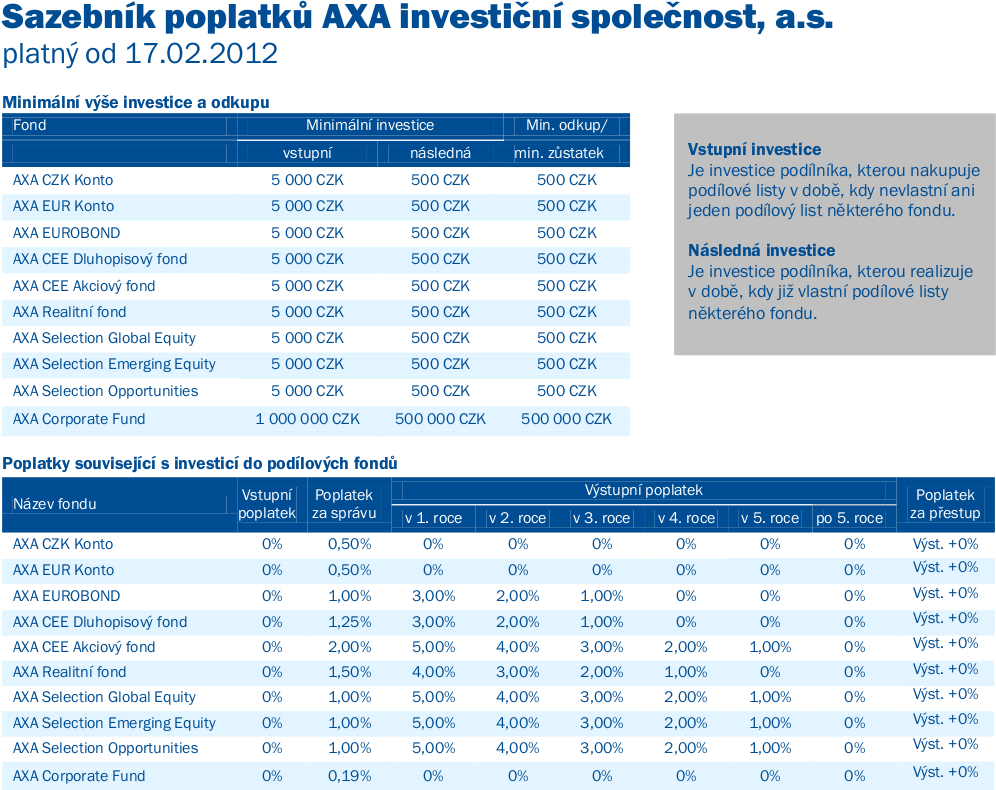
\includegraphics[width=0.8\textwidth]{axa_popl.png}			
			\end{center}
		\end{frame}
		\subsubsection{AXA CZK Konto}
			\begin{frame}{AXA CZK Konto}
				\begin{quote}
				Cílem investiční strategie je poskytnout podílníkům růst hodnoty jejich investice za podmínky, že celkový rizikový profil fondu minimalizuje možnost ztráty v horizontu 6 měsíců. Cíle je dosahováno investicemi do široce diverzifikovaného portfolia cenných papírů s fixním nebo variabilním úrokovým výnosem a aktivním řízením úrokového rizika.\footnote{\url{http://www.axa.cz/lide/podilove-fondy/czk-konto/popis}}
				\end{quote}
			\end{frame}
			\begin{frame}{AXA CZK Konto}
				\begin{center}
					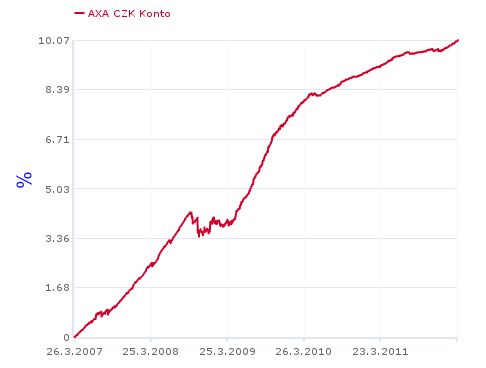
\includegraphics[width=0.7\textwidth]{axa_czk_konto.png}
				\end{center}							
				Výkon za 5 let 10.07\%, což je 1.93\% ročně, za poslední rok 0.8\%.
			\end{frame}
			\begin{frame}{AXA CEE Dluhopisový fond}
			\begin{quote}
				Fond investuje do dluhopisů emitentů všech kategorií:
				\begin{itemize}
			    \item dluhopisů nadnárodních institucí
			    \item státních dluhopisů
			    \item bankovních dluhopisů
			    \item dluhopisů obchodních společností
			    \item komunálních dluhopisů emitovaných v krajinách střední a východní Evropy\footnote{\url{http://www.axa.cz/lide/podilove-fondy/cee-dluhopisovy/popis}}	
    	  \end{itemize}
		  \end{quote}
		  Doporučeným investičním horizontem jsou minimálně 3 roky. Fond je určen pro střednědobé investice s mírou rizika i výnosem o něco výššími než u fondu peněžního trhu.
			\end{frame}
			\begin{frame}{AXA CEE Dluhopisový fond}
				\begin{center}
					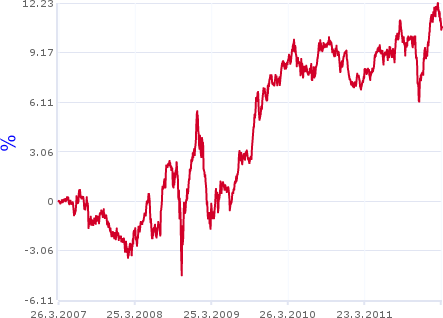
\includegraphics[width=0.7\textwidth]{axa_cee_dluh.png}
				\end{center}							
				Výkon za 5 let 10.73\%, což je 2.05\% ročně.\\
				Monhem vyšší volatilita.
			\end{frame}
			\begin{frame}{AXA CEE Akciový fond}
				\begin{quote}
				Cílem fondu je dosahovat co nejvyššího dlouhodobého zhodnocení investic. Majetek fondu je tvořený především akciemi společností, které jsou lídry ve svém odvětví v regionu střední a východní Evropy. Největší podíl na portfoliu mají české, polské a maďarské společnosti. Odvětvová struktura portfolia není omezená, významně se na ní ale podílí energetický, telekomunikační a finanční sektor. Investice jsou směřované také do odvětví farmacie či strojírenství.\footnote{\url{http://www.axa.cz/lide/podilove-fondy/cee-akciovy/popis}}
			\end{quote}
			Doporučeným investičním horizontem je minimálně 5 let. Fond pro ivestora slibuje vyskoké zhodnocení v dlouhém období, ale za cenu vysoké střednědobé volatility.
			\end{frame}
			\begin{frame}{AXA CEE Akciový fond}
				\begin{center}
					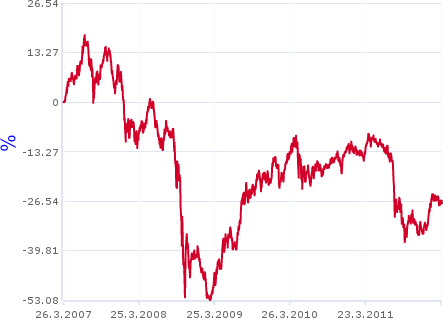
\includegraphics[width=0.7\textwidth]{axa_cee_akc.png}
				\end{center}							
				Za 5 let fond ztratil 27.11\% hodnoty, v době finanční krize dokonce 52.3\%.
			\end{frame}
	\subsection{Pioneer Asset Management, a.s. -- Rentier Invest}
	\begin{frame}{Pioneer Asset Management, a.s. -- Rentier Invest}
		Program tvoří 7 na sebe navazujících linií s postupně se snižující rizikovostí a výnosem.
		\begin{center}
			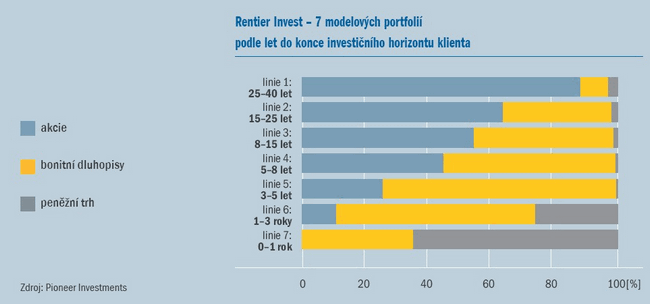
\includegraphics[width=0.9\textwidth]{graf_alokace_linii.png}
		\end{center}
	\end{frame}
	\begin{frame}{Rentier Invest}
		Minimálně je možno investovat poprvé 30 000 Kč, následně 10 000 Kč nebo pravidelně 1 000 Kč.
		\begin{center}
			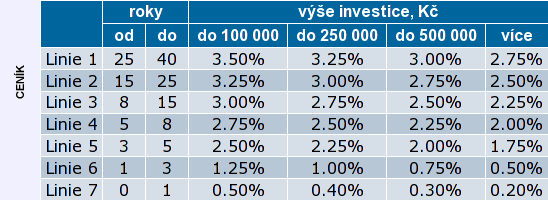
\includegraphics[width=0.9\textwidth]{ri_cost.png}
		\end{center}
	\end{frame}
		\begin{frame}{Rentier Invest}
		\begin{center}
			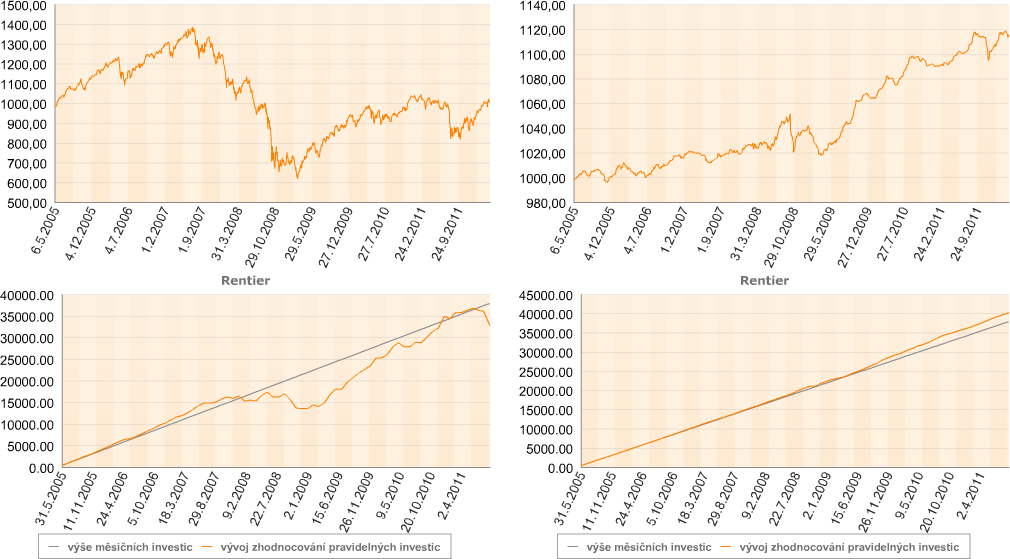
\includegraphics[width=1.0\textwidth]{ri_graf.png}
		\end{center}
		Linie 1 dosáhla za posledních 5 let ztráty 22.08\%, linie 7 zisku 9.27\%.
	\end{frame}
\end{document}